\documentclass{article}
\usepackage{graphicx} % Required for inserting images

\usepackage{float}
\restylefloat{table}

\title{Data Mining - assigment 1}
\author{Patryk Janiak, Patrick Molina, Marek Seget, \\ Mateusz Bernart, ChihabEddine Zitouni}
\date{March 2024}

\begin{document}

\maketitle

\section{Introduction}

The Titanic's sinking stands as one of the most notorious maritime disasters in history. On April 15, 1912, during its inaugural journey, the supposedly unsinkable RMS Titanic foundered after striking an iceberg. Tragically, the insufficient number of lifeboats led to the loss of 1502 lives out of the 2224 passengers and crew aboard.

\section{Description of the dataset}

Dataset includes passenger information like name, age, gender, socio-economic class, etc. and most importantly whether the passenger survived the sinking. 

\section{Description of the input features}

\begin{table}[H]
\begin{tabular}{p{0.2\linewidth} | p{0.73\linewidth}}
\hline
Feature  & Description \\
\hline
pclass   & Ticket class; can be 1, 2 and 3 meaning respectively 1st, 2nd and 3rd class \\
sex      & Sex of the passenger; can be male or female \\
age      & Age given in years \\
sibsp    & Number of siblings or spouses aboard the Titanic \\
parch    & Number of parents or children aboard the Titanic \\
ticket   & Ticket number \\
fare     & Passenger fare \\
cabin    & Cabin number \\
embarked & Port where the passenger had embarked on the Titanic; can be C, Q and S for respectively Cherbourg, Queenstown and Southampton \\
\hline
\end{tabular}
\end{table}

\section{Exploratory analysis of the input features}

\begin{figure}[H]
    \centering
    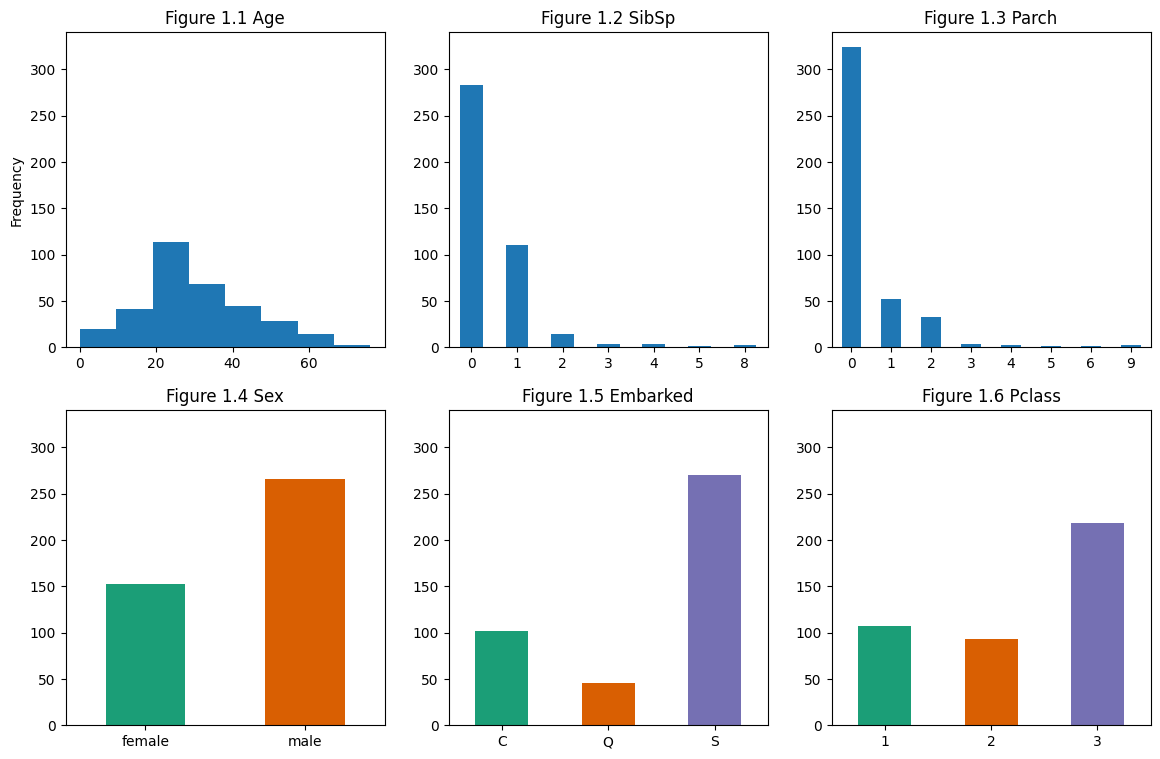
\includegraphics[width=1\linewidth]{input_features.png}
    \caption{Analysis of the input features}
    \label{fig:Analysis of the input features}
\end{figure}

As we can see in Figure 1.1 the majority of the people on board were in their twenties and thirties. In Figure 1.2 it is clear that most did not have any siblings nor spouses on the ship which is similar to what can be observed in Figure 1.3 where the number of people with parents or children is less than 25\%. There is almost twice as many males than females shown in Figure 1.4. As seen in Figure 1.5 most people embarked from Southampton followed by Cherbourg and Queenstown. The Figure 1.6 shows the distribution of passenger classes.

\section{Preprocessing techniques used in the assignment}

\subsection{Handling missing values}

Dropped columns with no relevant information and removed rows with missing values, considering the importance of features in the dataset.

\subsection{Encoding categorical variables}

Converted categorical variables like 'Sex' and 'Embarked' into numerical labels for machine learning algorithms to process.

\subsection{Normalization and standarization}

We tested both preprocessing techniques and we decided to perform the data scaling using StandardScaler over the MinMaxScaler.

\section{Description of the output features}

In the dataset there is only one output feature - Survived. It is either 0 or 1 whenever the passenger perished or survived.

\section{Exploratory analysis of the output features}

\begin{figure}[H]
    \centering
    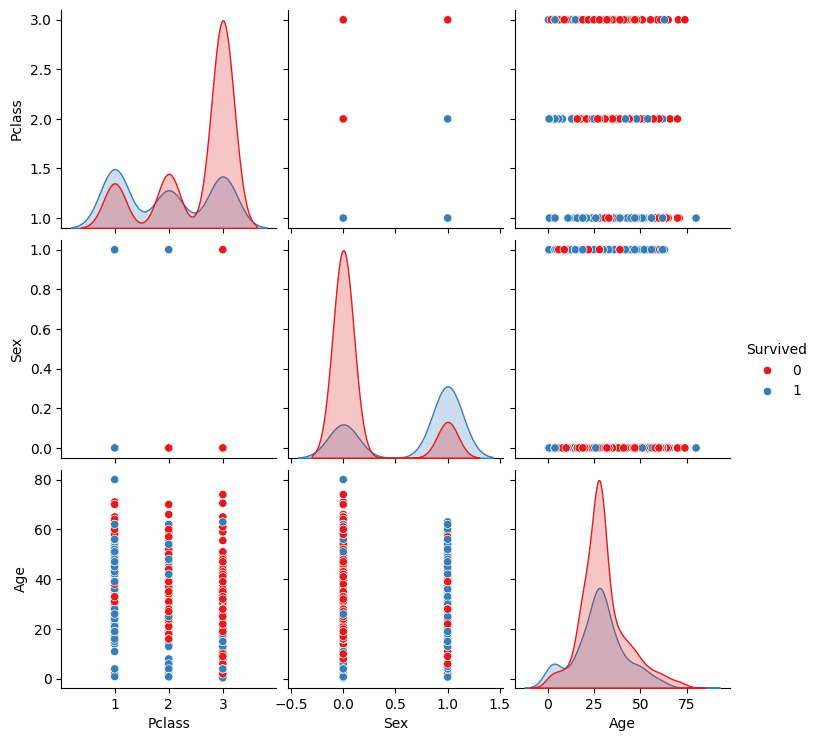
\includegraphics[width=1\linewidth]{output_features.png}
    \caption{Relational analysis of selected input features and the output feature}
    \label{fig:pairwise-relationships analysis}
\end{figure}

In Figure 2 we can see patterns emerge showing us that there exist a predictive model that is able to classify passenger's survival.

\section{Conclusions}

We decided to use RFE with Logistic Regression and Random Forest Classifier to select the most important features for prediction. After that we applied PCA to reduce the dimensionality of the dataset while retaining important information, creating new features.

This allowed us to train machine learning models (Logistic Regression, SVC) on the training dataset with selected and extracted features. We have evaluated the models' performance on the validation set using metrics such as accuracy and classification report.

To finalize we checked the trained models to predict the survival outcomes of passengers in the test set, who did not have their survival status provided.

\begin{table}[H]
\begin{tabular}{p{0.3\linewidth} | p{0.63\linewidth}}
\hline
Classifier  & Accuracy on the test dataset\\
\hline
SVC                  & 90.93\% \\
Random Forest        & 85.49\% \\
Logistic Regression  & 90.93\% \\
\hline
\end{tabular}
\end{table}

\end{document}
